\section{Research Method}
\label{sec:research-method}

The research method we're using are not traditionally adopted in most current academic environments.
Since the method is basically always following up with the latest and better way of thinking.
This attainment of doing is chosen because we need to constantly adjusting to the condition along the time, not just in the first phase.

To make things even leaner and more effective, we use agile methodologies to conduct the development.
Agile itself is a time boxed, iterative approact to software delivery that builds software incrementally from the start of the project, instead of trying to deliver it all at once near the end.
It works by breaking projects down into little bits of user functionality called user stories, prioritizing them, and then continuously delivering them in short two week cycles called iterations.~\autocite{Rasmusson2015Agile}
Therefore, we don't risk in creating a big or even a thing that small for a long time.
Because we iterate the result, coming back again as like a beginning.
Essentially, we learn and relearn what we could have done in each iteration process.
In a process matter of sense, analysis, design, development/coding, and testing are continuous activities.
In addition, there are a lot of other aspects that required:

\begin{easylist}
& Development itself is iterative
& Planning is adaptive
& The scope variables may vary
& Requirements can change over time
& Working software is the primary measure of success
& and other leaned segments to consider
\end{easylist}

Agile methodologies also heavily corresponds with building a \ac{MVP}\index{Minimum Viable Product} or we can also called it a \ac{MWT}\index{Minimum Working Thing}. Shortly defined, each elements of \ac{MVP} are:

\begin{description}
  \item[Minimum] The least or smallest amount possible.
  \item[Viable] Capable of working successfully.
  \item[Product] An article or substance that is created or refined for sale.~\autocite{Montgomery2013MWT}
\end{description}

We can also illustrate it as creating a vehicle with two different steps.

\begin{figure}[htb]
    \centering
    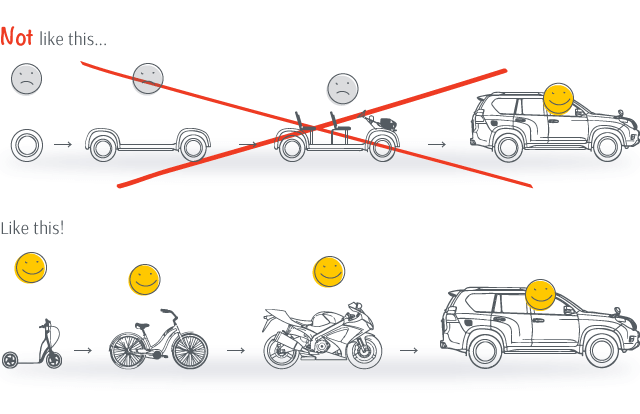
\includegraphics[width=\textwidth]{\dir/include/mvp-1}
    \caption[MVP illustrated]{MVP illustrated with only one usable product and some incremental products~\autocite{Mercury2014MVP}}
    \label{fig:method:mvp-1}
\end{figure}

As in figure \autoref{fig:method:mvp-1}, the first one is a need to take a lot of steps of before finally finished the final usable product.
The second one is an incremental steps of creating the usable product, until it's final yet to be usable as visioned and planned.
It can be seen that the second approach is more appealing and effective than the first.

\begin{figure}[htb]
    \centering
    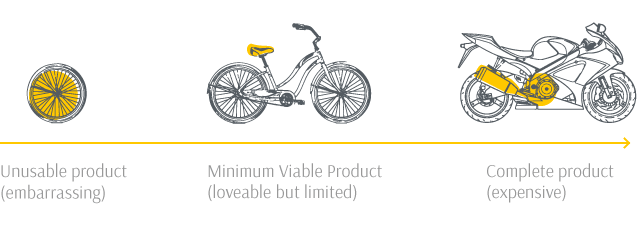
\includegraphics[width=\textwidth]{\dir/include/mvp-2}
    \caption[MVP compared]{MVP compared with unusable and complete product~\autocite{Mercury2014MVP}}
    \label{fig:method:mvp-2}
\end{figure}

Also as in figure \autoref{fig:method:mvp-2}, \ac{MVP} is compared with unusable product and complete product.
In this context, \ac{MVP} is ideally more balanced and preferable than the others.
More than that, if there is more effort and time, we can build a \ac{MLP}\index{Minimum Loveable Product}.
Which is an \ac{MVP} but taken beyond a working thing, which the customer will actually love using.
It's an embodiment of a production ready and could potentially get a customer or lots of them.
The thing that matters and can be used well.

Because thesis procedure has a very limited time, we can only took the limit until it is viable enough yet basically usable.
We first only focus on the main basic features.
Yet, the development will always be continued further as a product of startup.
The code and supporting commpents themself will be released as an open source project.
So with the backing help of company and endorsement of community, this could handed by a lot of people.

But then, which \ac{MVP} that is most required to be used?
We can determine that by using a business model tool called \ac{BMC}\index{Business Model Canvas}.
More details about \ac{BMC} is later described in \autoref{sec:bmc} and the resulting one is in \autoref{sec:bmc-satellid}.
Related to \ac{MVP}, \ac{BMC} includes the most important components which are Customer Segments and Value Propositions.
Customer Segments define for whom the MVP is built for.
And Value Propositions define what features the MVP need first and mainly.

In more technical side, the \ac{SDLC}\index{software development life cycle} of this software follows or tends to assist a software development principle called \ac{DRY}\index{don't repeat yourself},
which every piece of knowledge must have a single, unambiguous, authoritative representation within a system.~\autocite{Hunt1999Pragmatic}
The code then resulted in a cleaner and clearer structure.
In detail, this applied in database schemas even we use a very flexible document database.
As well as test plans, the build system, and documentation within or outside the code.
Applied also in the user interaction design, therefore there is a decreased amount of duplicated data that is accidentally created or not intended by users.
In addition to make the historical development process more well-organized and can be collaborative, the repository of the source code is managed using a \ac{VCS}\index{version control system} or \ac{SCM}\index{source code management} called Git\index{git} which later described in \autoref{sec:scm}.
\autoref{sec:problem-scope},
